% Ensure that you compile using XeLaTeX !!! PDFTex has problems with some of the packages used
\documentclass[12pt]{article}
\setlength\parindent{0pt}

\usepackage{parskip}
\usepackage[margin=0.5in]{geometry}
\usepackage{fullpage}
\usepackage{moresize}
\usepackage{graphicx}
\usepackage{caption}
\usepackage{subcaption}
\usepackage{float}
\usepackage{xcolor}
\usepackage{soul}
\usepackage{fontspec}
\setmainfont{Doulos SIL}

\begin{document}

\begin{center}
\textbf{{\color{violet}{\HUGE Monday, 22 June 2020\\}}}

\textbf{{\color{violet}{\HUGE ALL EXAMS\\}}}

\end{center}
\newpage

\begin{center}
\textbf{{\color{blue}{\HUGE START OF EXAM\\}}}

\textbf{{\color{blue}{\HUGE Student ID: 4066\\}}}

\textbf{{\color{blue}{\HUGE 2:20 - 2:40 PM\\}}}

\end{center}
\newpage

{\large Question 1}\\

Source: Day 9 Handout, Question 1\\

Explain why the concept of an alternation either is or is not useful for understanding this dataset.\\

\begin{figure}[H]
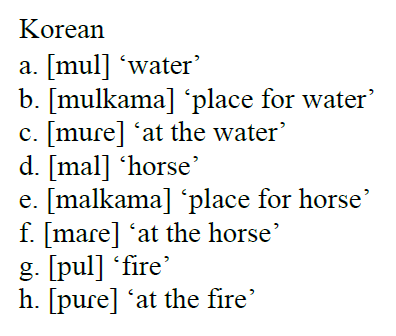
\includegraphics{../images/korean.png}
\end{figure}

\newpage

{\large Question 2}\\

Source: Final Exam Dataset\\

Explain what the basic phonological analysis of this dataset is, and what the key pieces of evidence are.\\

\begin{figure}[H]
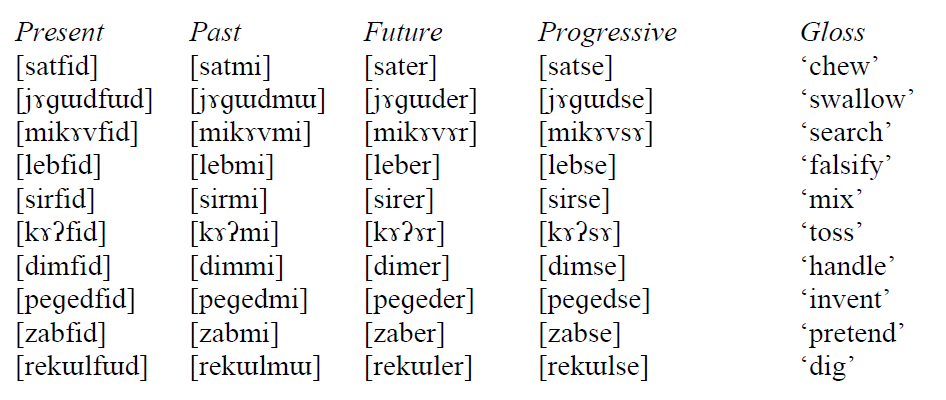
\includegraphics{../images/final_dataset.png}
\end{figure}

\newpage

{\large Question 3}\\

Source: Day 10 Discussion\\

Explain why the given feature's value varies across this set of sounds.\\

{[sonorant]}

alveolars


\newpage

{\large Question 4}\\

Source: Day 8 Handout, Question 7\\

Explain why each numbered, underlined statement is true or false. If it is false, explain one way that you could correct it.\\

We can look at the vertical location of the formants to determine something about the characteristics of individual speech sounds. For example, in the two spectrograms below, we can see that $^{22}$\ul{the first formant is higher in the spectrogram for sound 1 than it is for sound 2.} Because $^{23}$\ul{F1 is directly correlated with vowel height}, we know that $^{24}$\ul{the vowel pictured in sound 1 is a higher vowel than the one in sound 2}. For example, $^{25}$\ul{sound 1 might be an {[ɑ]} while sound 2 might be an {[i]}.}

\begin{figure}[H]
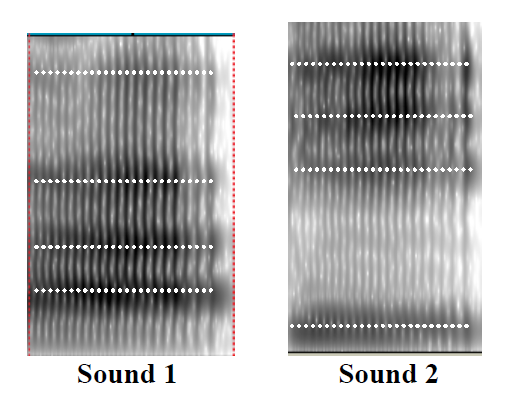
\includegraphics{../images/sound1a_sound2i.png}
\end{figure}

\newpage

{\large Question 5}\\

Source: Quiz 10, Question 3\\

Section 4.2 of chapter 13 in the Peng textbook presented an autosegmental analysis of Mende tone distribution. Explain why the form shown below should NOT be the UR for any morpheme in Mende.\\

\begin{figure}[H]
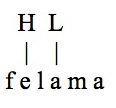
\includegraphics{../images/mende_junction_a.png}
\end{figure}

\newpage

{\large Question 6}\\

Source: Homework 5, Question 2\\

Explain why the insertion analysis is better than the deletion analysis for this dataset.\\

\begin{figure}[H]
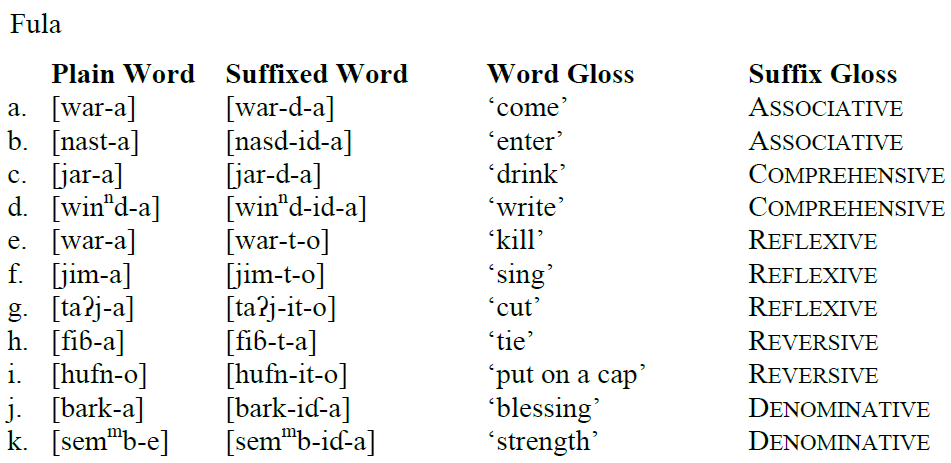
\includegraphics{../images/fula.png}
\end{figure}

\newpage

\begin{center}
\textbf{{\color{red}{\HUGE END OF EXAM}}}\\

\end{center}
\newpage

\begin{center}
\textbf{{\color{blue}{\HUGE START OF EXAM\\}}}

\textbf{{\color{blue}{\HUGE Student ID: 9246\\}}}

\textbf{{\color{blue}{\HUGE 2:40 - 3:00 PM\\}}}

\end{center}
\newpage

{\large Question 1}\\

Source: Day 11 Handout, Question 10\\

Explain why this structure either is or is not a correct application of the templatic-based approach to syllabification, using the provided template and assuming that syllabification proceeds from left to right.\\

\begin{figure}[H]
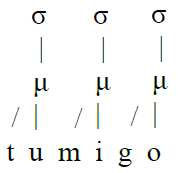
\includegraphics{../images/pengtemplate_tumigo_yes.png}
\end{figure}
\begin{figure}[H]
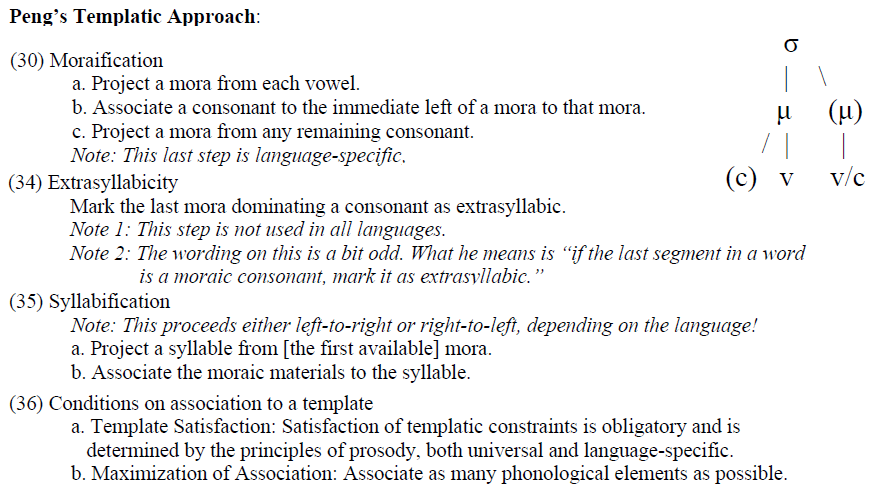
\includegraphics{../images/peng_template_withdiagram.png}
\end{figure}

\newpage

{\large Question 2}\\

Source: Final Exam Dataset\\

Give a good phonological description of the patterns in the dataset that should be analysed.\\

\begin{figure}[H]
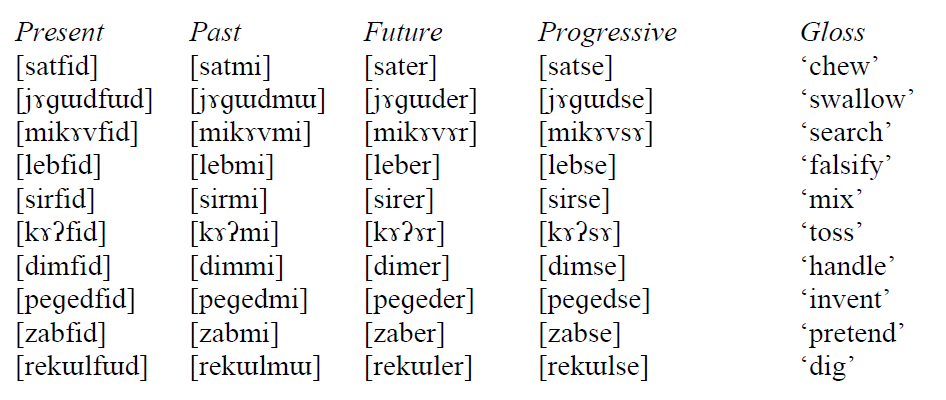
\includegraphics{../images/final_dataset.png}
\end{figure}

\newpage

{\large Question 3}\\

Source: Day 8 Handout, Question 7\\

Explain why each numbered, underlined statement is true or false. If it is false, explain one way that you could correct it.\\

Sound is an invisible phenomenon. Sound can travel through any substance, $^1$\ul{such as a liquid, solid, or a gas.} $^2$\ul{It involves the transfer of the matter in that substance} from one place to another.\\\\Sound is a particular kind of wave known as $^3$\ul{a compression wave}. $^4$\ul{When the molecules are really close together, we say they are ``rarefied'' and when they are really far apart, we say they are ``compressed.''}


\newpage

{\large Question 4}\\

Source: Day 12 Handout, Question 7\\

What would be a good description of the alternation in this dataset?\\

\begin{figure}[H]
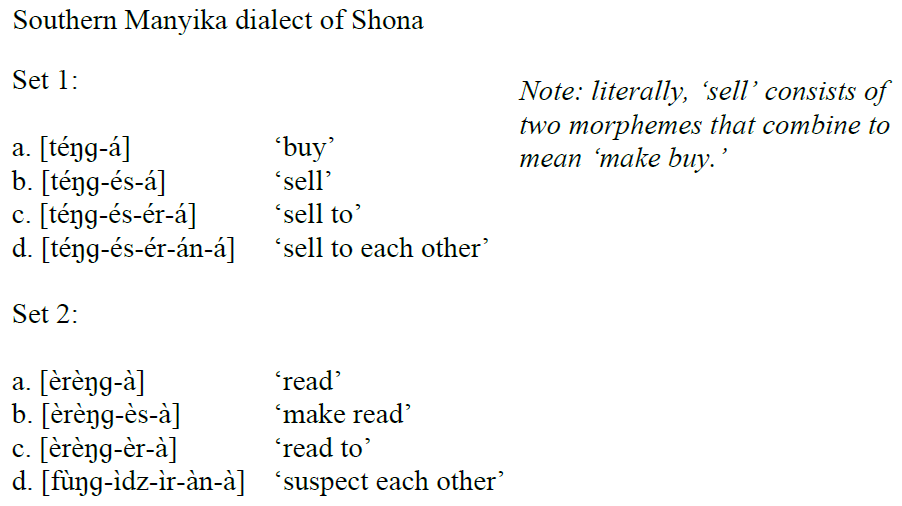
\includegraphics{../images/shona.png}
\end{figure}

\newpage

{\large Question 5}\\

Source: Day 9 Handout, Question 5\\

Explain which morpheme(s) in this dataset alternate and how that helps you do a phonological analysis.\\

\begin{figure}[H]
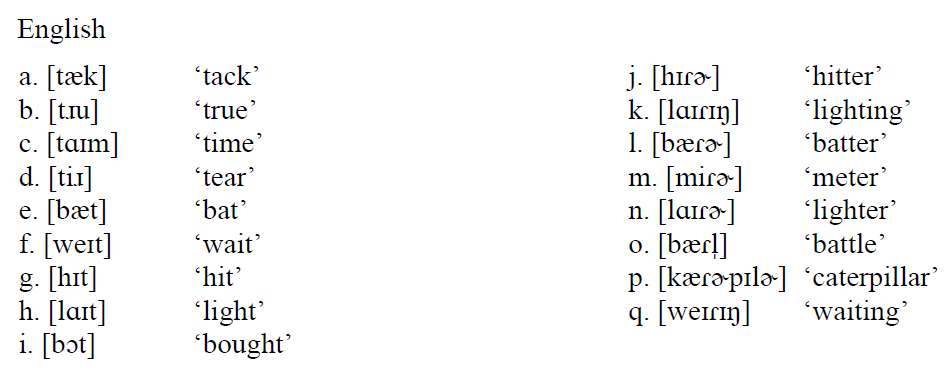
\includegraphics{../images/english_t_flap.png}
\end{figure}

\newpage

{\large Question 6}\\

Source: Quiz 8, Question 6\\

Explain why this is an incorrect statement.\\

Nasal consonants are {[+continuant]}, because you can continue to make the sound for a long period of time (until you run out of breath).


\newpage

\begin{center}
\textbf{{\color{red}{\HUGE END OF EXAM}}}\\

\end{center}
\newpage

\begin{center}
\textbf{{\color{blue}{\HUGE START OF EXAM\\}}}

\textbf{{\color{blue}{\HUGE Student ID: 4090\\}}}

\textbf{{\color{blue}{\HUGE 3:00 - 3:20 PM\\}}}

\end{center}
\newpage

{\large Question 1}\\

Source: Day 9 Handout, Question 1\\

Explain why the concept of an alternation either is or is not useful for understanding this dataset.\\

\begin{figure}[H]
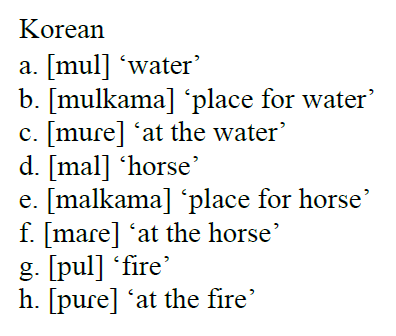
\includegraphics{../images/korean.png}
\end{figure}

\newpage

{\large Question 2}\\

Source: Final Exam Dataset\\

Explain what the underlying representation of these morphemes would be and why.\\

`invent', `progressive'

\begin{figure}[H]
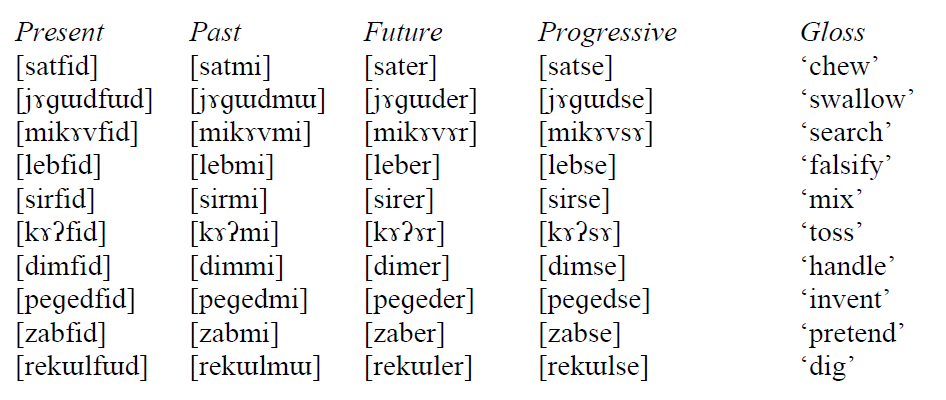
\includegraphics{../images/final_dataset.png}
\end{figure}

\newpage

{\large Question 3}\\

Source: Day 11 Handout, Question 6\\

Explain why this structure either is or is not a correct application of the rule-based approach to syllabification, assuming that both the onset rule and the coda rule apply in this language, and the onset rule comes before the coda rule.\\

\begin{figure}[H]
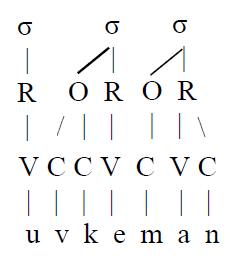
\includegraphics{../images/pengrules_uvkeman_yes.png}
\end{figure}
\begin{figure}[H]
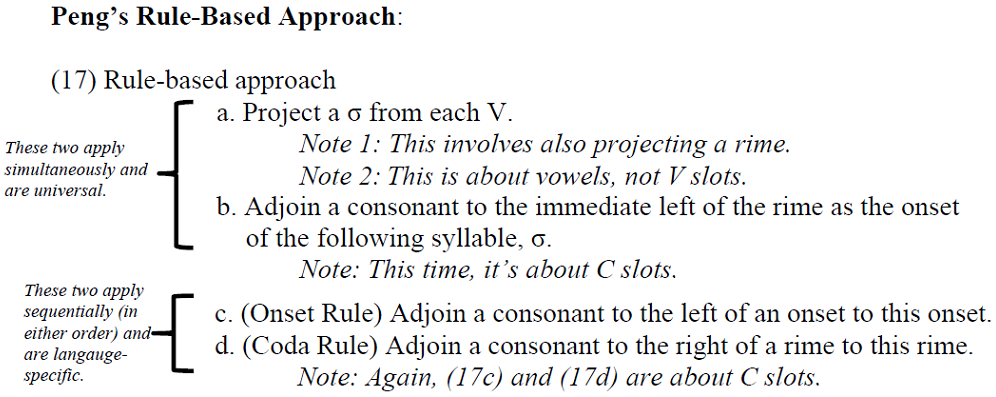
\includegraphics{../images/peng_rules.png}
\end{figure}

\newpage

{\large Question 4}\\

Source: Day 8 Handout, Question 1\\

Explain what (if anything) the letter below represents on this waveform.\\

A

\begin{figure}[H]
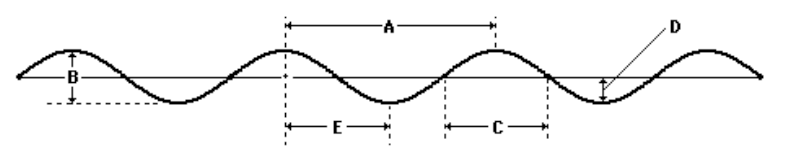
\includegraphics{../images/sinusoid.png}
\end{figure}

\newpage

{\large Question 5}\\

Source: Day 12 Handout, Question 5\\

Explain which of the three rules will apply to the form given below, and whether each of those rules would have an effect or not.\\

Peng’s Tone-Mapping Procedure for Mende: \begin{enumerate} \item L-to-R association: Associate the first tone to the first TBU, the second tone to the second TBU, and so on, until all tones or all TBUS are exhausted. \item Last-TBU Linking: Associate any remaining unlinked tones to the last TBU. \item Last-Tone Linking: Associate the last tone to any TBU without a tone. \end{enumerate}

\begin{figure}[H]
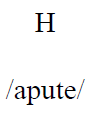
\includegraphics{../images/mendetone_b.png}
\end{figure}

\newpage

{\large Question 6}\\

Source: Day 10 Handout, Question 6 (Day 7 Handout, Question 7)\\

Explain how you should use phonological features to combine these rules.\\

/s/ → {[ʃ]} / \_\_ {[i]} \\/z/ → {[dʒ]} / \_\_ {[i]}

\begin{figure}[H]
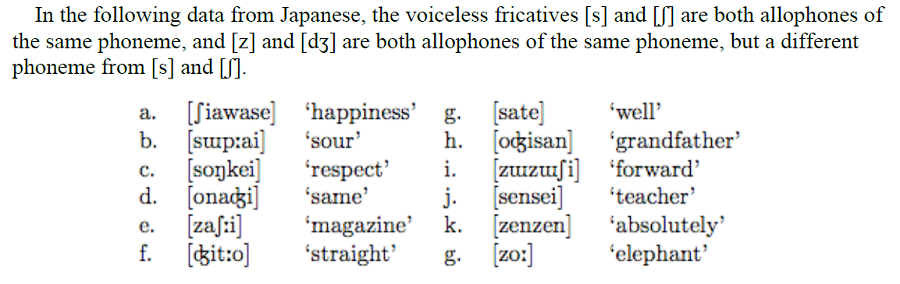
\includegraphics{../images/japanese.png}
\end{figure}

\newpage

\begin{center}
\textbf{{\color{red}{\HUGE END OF EXAM}}}\\

\end{center}
\newpage

\begin{center}
\textbf{{\color{blue}{\HUGE START OF EXAM\\}}}

\textbf{{\color{blue}{\HUGE Student ID: 1956\\}}}

\textbf{{\color{blue}{\HUGE 3:20 - 3:40 PM\\}}}

\end{center}
\newpage

{\large Question 1}\\

Source: Quiz 10, Question 3\\

Section 4.2 of chapter 13 in the Peng textbook presented an autosegmental analysis of Mende tone distribution. Explain why the form shown below should NOT be the UR for any morpheme in Mende.\\

\begin{figure}[H]
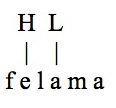
\includegraphics{../images/mende_junction_a.png}
\end{figure}

\newpage

{\large Question 2}\\

Source: Final Exam Dataset\\

Explain what the underlying representation of these morphemes would be and why.\\

`invent', `progressive'

\begin{figure}[H]
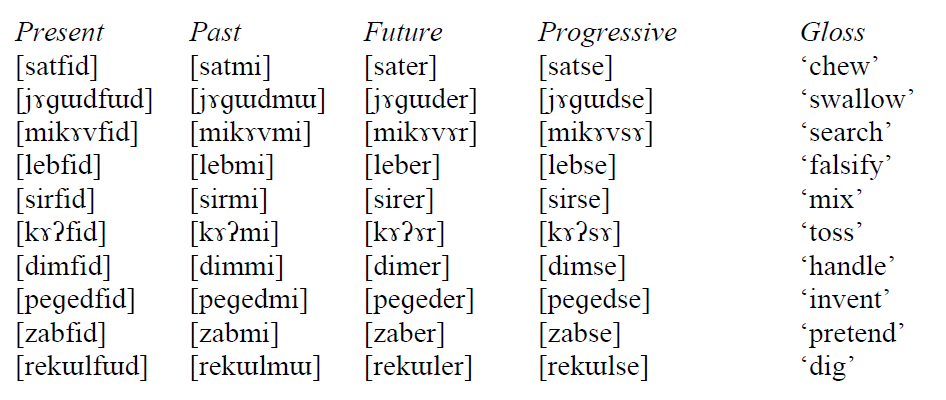
\includegraphics{../images/final_dataset.png}
\end{figure}

\newpage

{\large Question 3}\\

Source: Day 8 Handout, Question 7\\

Explain why each numbered, underlined statement is true or false. If it is false, explain one way that you could correct it.\\

$^{10}$\ul{Frequency is inversely related to pitch: high frequencies correspond to low pitches, and low frequencies correspond to high pitches.} Finally, there is the amplitude of the wave. $^{11}$\ul{The amplitude tells you how much pressure the molecules are under at any particular time.} $^{12}$\ul{The auditory correlate of amplitude is intensity}; this is a measure of perceived pressure.\\\\$^{13}$\ul{In speech, air is set in vibrating motion by the lungs, so the lungs} are the source of most speech sounds.


\newpage

{\large Question 4}\\

Source: Day 11 Handout, Question 14\\

How does syllabification play a role in the analysis of the phonological relationship between tense and lax high vowels in Quebec French?\\

\begin{figure}[H]
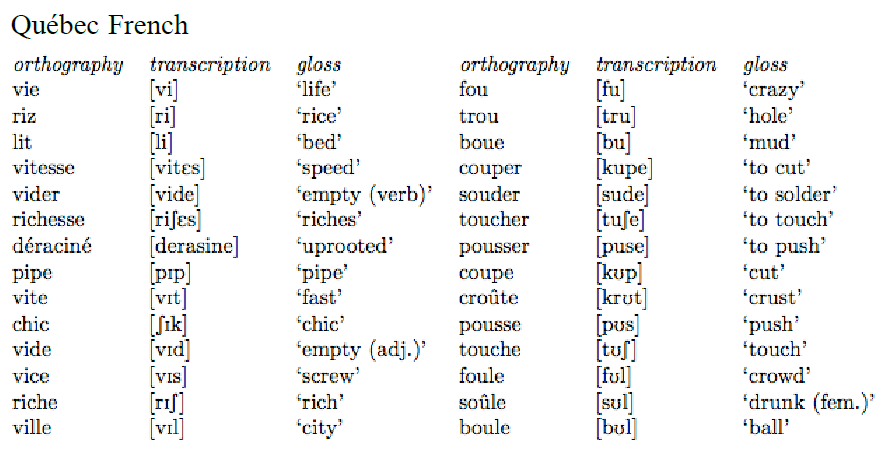
\includegraphics{../images/quebecfrench.png}
\end{figure}

\newpage

{\large Question 5}\\

Source: Day 9 Handout, Question 5\\

Explain which morpheme(s) in this dataset alternate and how that helps you do a phonological analysis.\\

\begin{figure}[H]
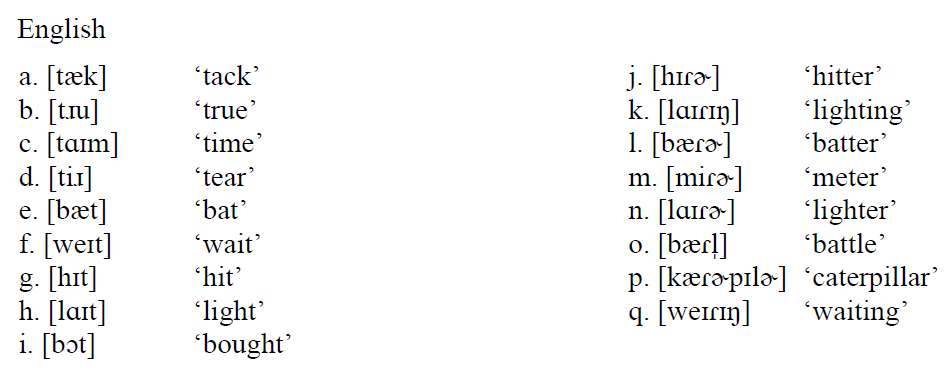
\includegraphics{../images/english_t_flap.png}
\end{figure}

\newpage

{\large Question 6}\\

Source: Day 10 Discussion\\

Explain why the given feature's value varies across this set of sounds.\\

{[voice]}

glottalized obstruents


\newpage

\begin{center}
\textbf{{\color{red}{\HUGE END OF EXAM}}}\\

\end{center}
\newpage

\begin{center}
\textbf{{\color{blue}{\HUGE START OF EXAM\\}}}

\textbf{{\color{blue}{\HUGE Student ID: 3737\\}}}

\textbf{{\color{blue}{\HUGE 3:40 - 4:00 PM\\}}}

\end{center}
\newpage

{\large Question 1}\\

Source: Day 11 Handout, Question 5\\

Explain why this template either does or does not allow syllables of this type to occur.\\

CCV

\begin{figure}[H]
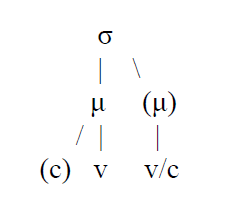
\includegraphics{../images/ponapean_syllabletemplate.png}
\end{figure}

\newpage

{\large Question 2}\\

Source: Final Exam Dataset\\

Explain what the underlying representation of these morphemes would be and why.\\

`invent', `progressive'

\begin{figure}[H]
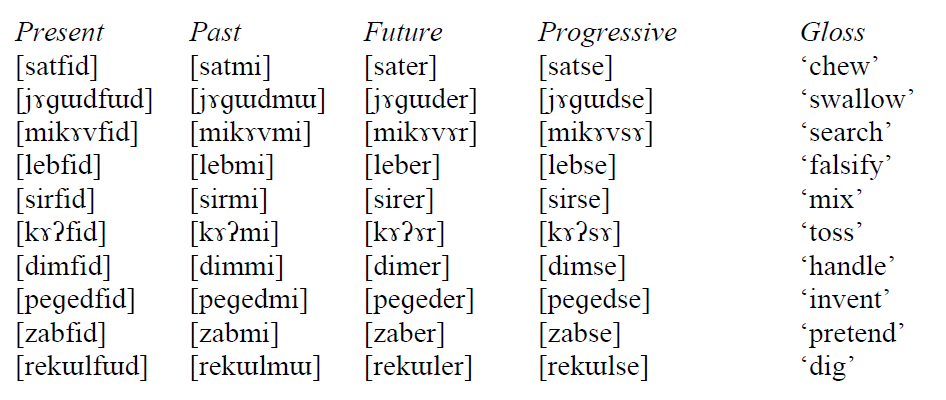
\includegraphics{../images/final_dataset.png}
\end{figure}

\newpage

{\large Question 3}\\

Source: Day 12 Handout, Question 5\\

Explain which of the three rules will apply to the form given below, and whether each of those rules would have an effect or not.\\

Peng’s Tone-Mapping Procedure for Mende: \begin{enumerate} \item L-to-R association: Associate the first tone to the first TBU, the second tone to the second TBU, and so on, until all tones or all TBUS are exhausted. \item Last-TBU Linking: Associate any remaining unlinked tones to the last TBU. \item Last-Tone Linking: Associate the last tone to any TBU without a tone. \end{enumerate}

\begin{figure}[H]
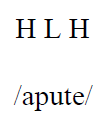
\includegraphics{../images/mendetone_a.png}
\end{figure}

\newpage

{\large Question 4}\\

Source: Day 8 Handout, Question 3\\

Explain what you see in the spectrogram that tells you about the properties of the sounds in the pictured word.\\

\begin{figure}[H]
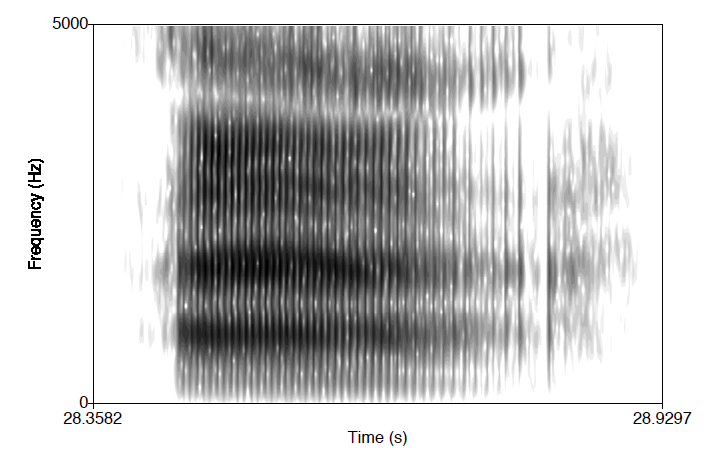
\includegraphics{../images/spectrogram_aaah.png}
\end{figure}

\newpage

{\large Question 5}\\

Source: Day 10 Discussion\\

Explain why the given feature's value varies across this set of sounds.\\

{[voice]}

glottalized obstruents


\newpage

{\large Question 6}\\

Source: Day 9 Handout, Question 3\\

Explain which morpheme(s) in this dataset alternate and how that helps you do a phonological analysis.\\

\begin{figure}[H]
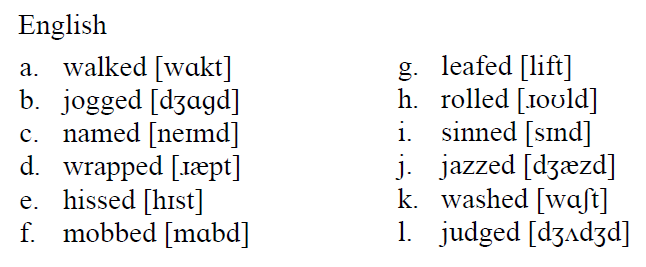
\includegraphics{../images/english_past.png}
\end{figure}

\newpage

\begin{center}
\textbf{{\color{red}{\HUGE END OF EXAM}}}\\

\end{center}
\newpage

\begin{center}
\textbf{{\color{blue}{\HUGE START OF EXAM\\}}}

\textbf{{\color{blue}{\HUGE Student ID: 4465\\}}}

\textbf{{\color{blue}{\HUGE 4:00 - 4:20 PM\\}}}

\end{center}
\newpage

{\large Question 1}\\

Source: Day 11 Handout, Question 12\\

Explain why what you’re analyzing in the following dataset either is or is not an alternation.\\

\begin{figure}[H]
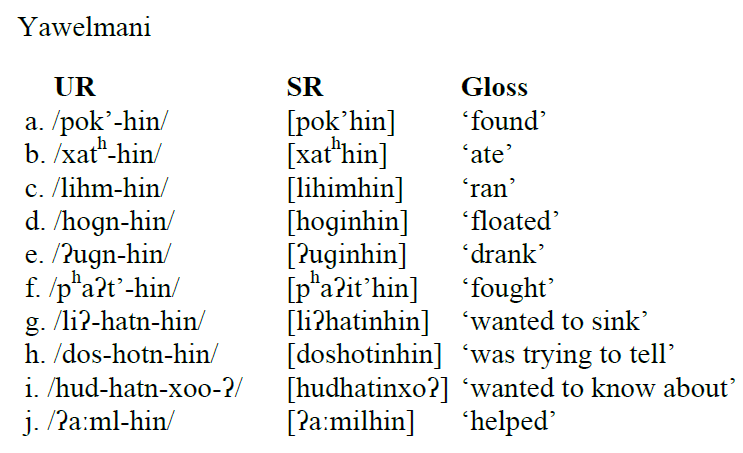
\includegraphics{../images/yawelmani.png}
\end{figure}

\newpage

{\large Question 2}\\

Source: Final Exam Dataset\\

Explain what the underlying representation of these morphemes would be and why.\\

`search', `present'

\begin{figure}[H]
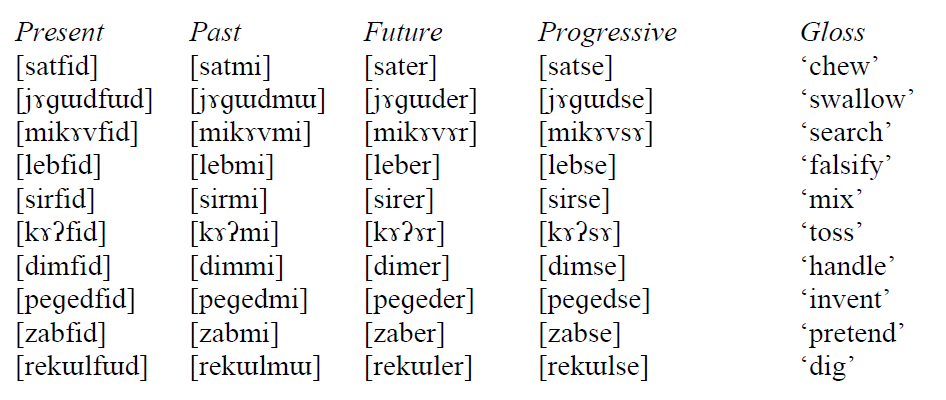
\includegraphics{../images/final_dataset.png}
\end{figure}

\newpage

{\large Question 3}\\

Source: Day 10 Handout, Question 6 (Homework 4, Question 2)\\

Explain how you should use phonological features in this rule. Which parts of the rule should include features, and what features might they be? You don't have to give an exact set of features, but what kinds of features would be involved?\\

/n/ → ∅ / {[m]} \_\_ \#

\begin{figure}[H]
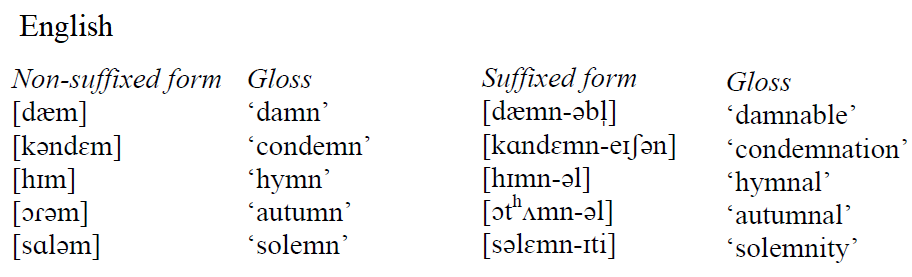
\includegraphics{../images/english_stemalternations.png}
\end{figure}

\newpage

{\large Question 4}\\

Source: Day 11 Handout, Question 10\\

Explain why this structure either is or is not a correct application of the templatic-based approach to syllabification, using the provided template and assuming that syllabification proceeds from left to right.\\

\begin{figure}[H]
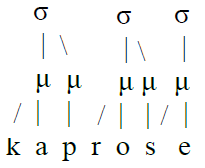
\includegraphics{../images/pengtemplate_kaprosse_yes.png}
\end{figure}
\begin{figure}[H]
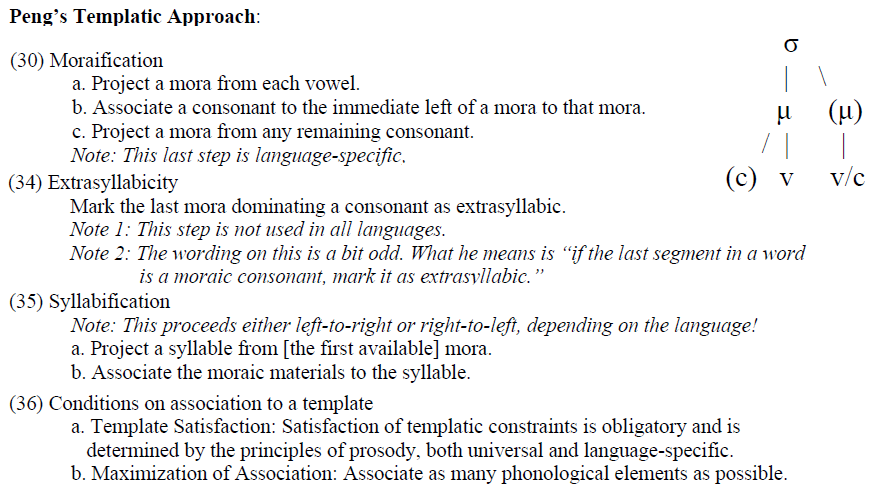
\includegraphics{../images/peng_template_withdiagram.png}
\end{figure}

\newpage

{\large Question 5}\\

Source: Day 12 Handout, Question 5\\

Explain which of the three rules will apply to the form given below, and whether each of those rules would have an effect or not.\\

Peng’s Tone-Mapping Procedure for Mende: \begin{enumerate} \item L-to-R association: Associate the first tone to the first TBU, the second tone to the second TBU, and so on, until all tones or all TBUS are exhausted. \item Last-TBU Linking: Associate any remaining unlinked tones to the last TBU. \item Last-Tone Linking: Associate the last tone to any TBU without a tone. \end{enumerate}

\begin{figure}[H]
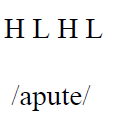
\includegraphics{../images/mendetone_d.png}
\end{figure}

\newpage

{\large Question 6}\\

Source: Day 8 Handout, Question 1\\

Explain what (if anything) the letter below represents on this waveform.\\

D

\begin{figure}[H]
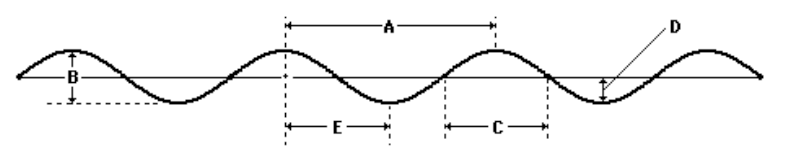
\includegraphics{../images/sinusoid.png}
\end{figure}

\newpage

\begin{center}
\textbf{{\color{red}{\HUGE END OF EXAM}}}\\

\end{center}
\newpage

\begin{center}
\textbf{{\color{blue}{\HUGE START OF EXAM\\}}}

\textbf{{\color{blue}{\HUGE Student ID: 9376\\}}}

\textbf{{\color{blue}{\HUGE 4:20 - 4:40 PM\\}}}

\end{center}
\newpage

{\large Question 1}\\

Source: Day 8 Handout, Question 1\\

Explain what (if anything) the letter below represents on this waveform.\\

C

\begin{figure}[H]
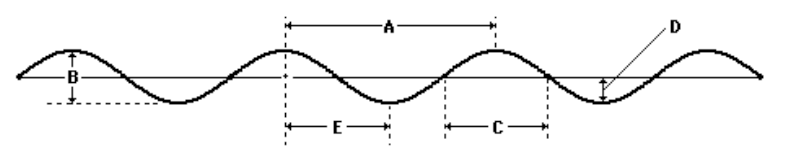
\includegraphics{../images/sinusoid.png}
\end{figure}

\newpage

{\large Question 2}\\

Source: Day 12 Handout, Question 5\\

Explain which of the three rules will apply to the form given below, and whether each of those rules would have an effect or not.\\

Peng’s Tone-Mapping Procedure for Mende: \begin{enumerate} \item L-to-R association: Associate the first tone to the first TBU, the second tone to the second TBU, and so on, until all tones or all TBUS are exhausted. \item Last-TBU Linking: Associate any remaining unlinked tones to the last TBU. \item Last-Tone Linking: Associate the last tone to any TBU without a tone. \end{enumerate}

\begin{figure}[H]
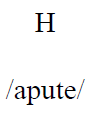
\includegraphics{../images/mendetone_b.png}
\end{figure}

\newpage

{\large Question 3}\\

Source: Final Exam Dataset\\

Explain what the underlying representation of these morphemes would be and why.\\

`search', `present'

\begin{figure}[H]
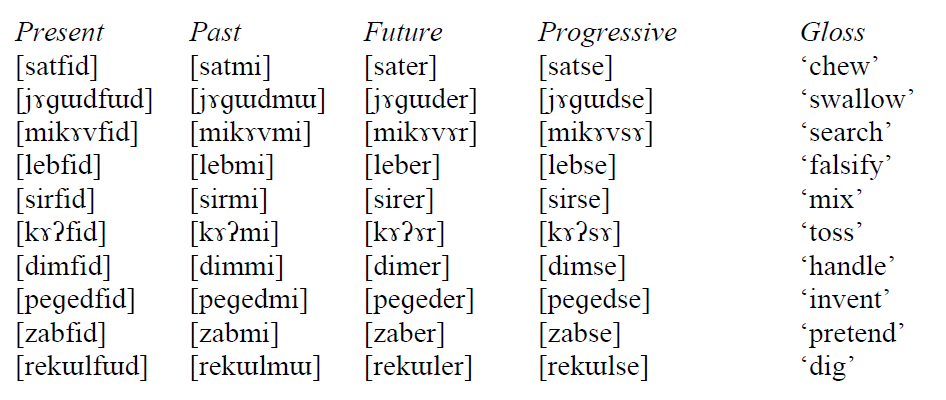
\includegraphics{../images/final_dataset.png}
\end{figure}

\newpage

{\large Question 4}\\

Source: Day 9 Handout, Question 5\\

Explain which morpheme(s) in this dataset alternate and how that helps you do a phonological analysis.\\

\begin{figure}[H]
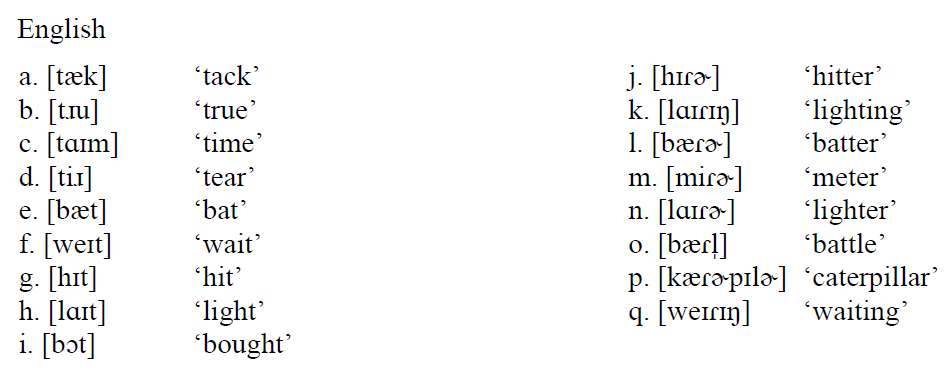
\includegraphics{../images/english_t_flap.png}
\end{figure}

\newpage

{\large Question 5}\\

Source: Day 11 Handout, Question 14\\

How does syllabification play a role in the analysis of the phonological relationship between tense and lax high vowels in Quebec French?\\

\begin{figure}[H]
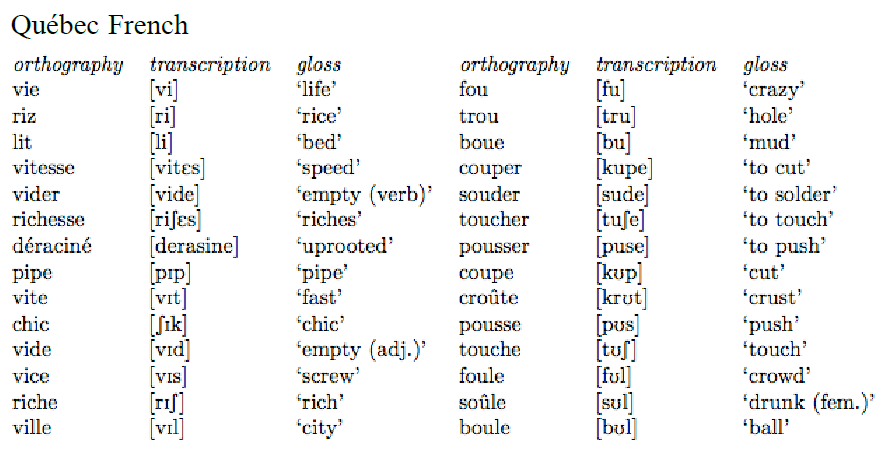
\includegraphics{../images/quebecfrench.png}
\end{figure}

\newpage

{\large Question 6}\\

Source: Quiz 8, Question 6\\

Explain why this is an incorrect statement.\\

Nasal consonants are {[+continuant]} because they lack a central occlusion in the vocal tract.


\newpage

\begin{center}
\textbf{{\color{red}{\HUGE END OF EXAM}}}\\

\end{center}
\newpage

\begin{center}
\textbf{{\color{blue}{\HUGE START OF EXAM\\}}}

\textbf{{\color{blue}{\HUGE Student ID: empty\\}}}

\textbf{{\color{blue}{\HUGE 4:40 - 5:00 PM\\}}}

\end{center}
\newpage

\begin{center}
\textbf{{\color{blue}{\HUGE START OF EXAM\\}}}

\textbf{{\color{blue}{\HUGE Student ID: 3347\\}}}

\textbf{{\color{blue}{\HUGE 5:00 - 5:20 PM\\}}}

\end{center}
\newpage

{\large Question 1}\\

Source: Quiz 10, Question 3\\

Section 4.2 of chapter 13 in the Peng textbook presented an autosegmental analysis of Mende tone distribution. Explain why the form shown below should NOT be the UR for any morpheme in Mende.\\

\begin{figure}[H]
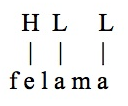
\includegraphics{../images/mende_junction_c.png}
\end{figure}

\newpage

{\large Question 2}\\

Source: Final Exam Dataset\\

Explain what the underlying representation of these morphemes would be and why.\\

`invent', `progressive'

\begin{figure}[H]
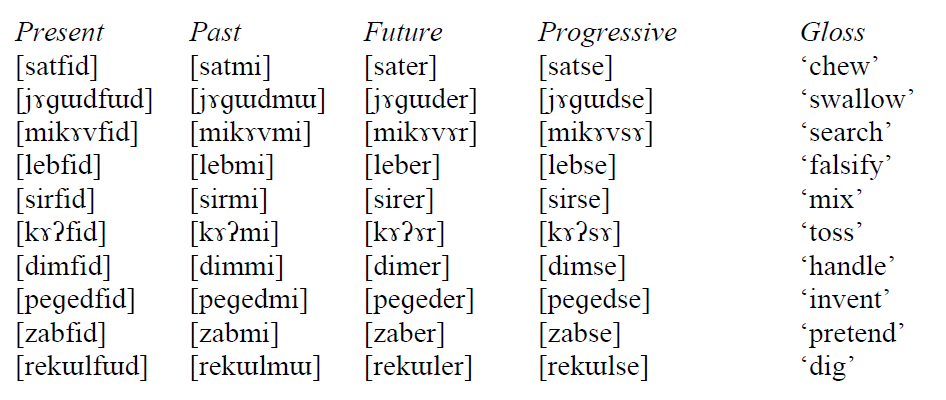
\includegraphics{../images/final_dataset.png}
\end{figure}

\newpage

{\large Question 3}\\

Source: Quiz 8, Question 3\\

Explain why this featural specification either does or does not match the given sound.\\

{[+consonantal]}, {[+sonorant]}

{[m]}


\newpage

{\large Question 4}\\

Source: Day 9 Handout, Question 3\\

Explain which morpheme(s) in this dataset alternate and how that helps you do a phonological analysis.\\

\begin{figure}[H]
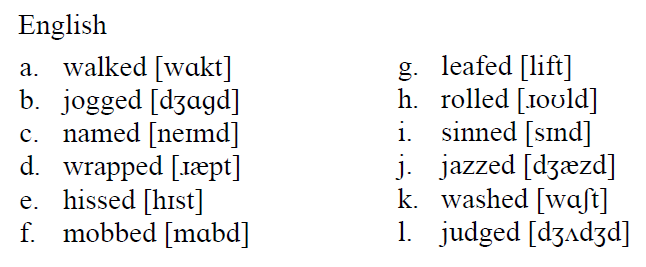
\includegraphics{../images/english_past.png}
\end{figure}

\newpage

{\large Question 5}\\

Source: Day 11 Handout, Question 6\\

Explain why this structure either is or is not a correct application of the rule-based approach to syllabification, assuming that both the onset rule and the coda rule apply in this language, and the onset rule comes before the coda rule.\\

\begin{figure}[H]
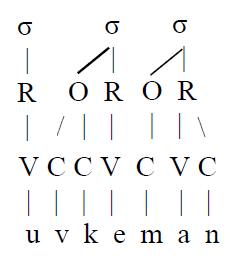
\includegraphics{../images/pengrules_uvkeman_yes.png}
\end{figure}
\begin{figure}[H]
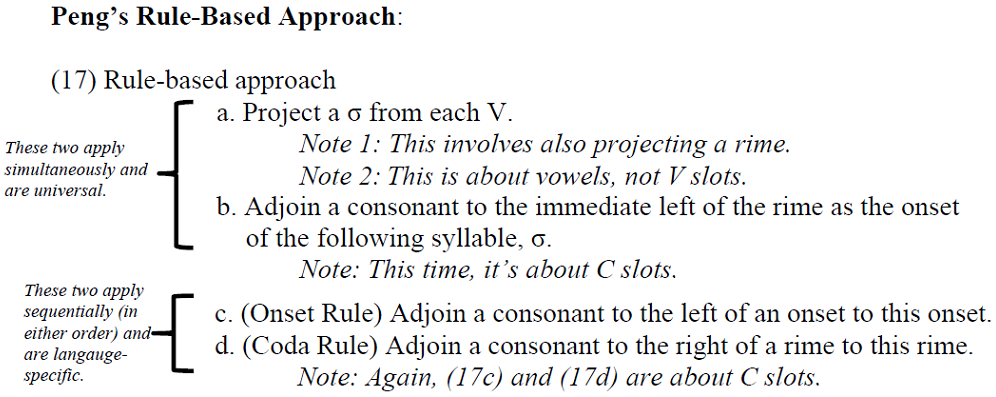
\includegraphics{../images/peng_rules.png}
\end{figure}

\newpage

{\large Question 6}\\

Source: Quiz 6, Question 2\\

Explain what you see in the spectrogram that tells you about the properties of the sounds in the pictured word.\\

\begin{figure}[H]
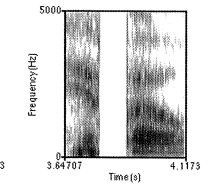
\includegraphics{../images/spectrogram_hippo.png}
\end{figure}

\newpage

\begin{center}
\textbf{{\color{red}{\HUGE END OF EXAM}}}\\

\end{center}
\newpage

\begin{center}
\textbf{{\color{blue}{\HUGE START OF EXAM\\}}}

\textbf{{\color{blue}{\HUGE Student ID: 3420\\}}}

\textbf{{\color{blue}{\HUGE 5:20 - 5:40 PM\\}}}

\end{center}
\newpage

{\large Question 1}\\

Source: Quiz 10, Question 1\\

Section 4.2 of chapter 13 in the Peng textbook presented an autosegmental analysis of Mende tone distribution. Explain why the form shown below should NOT be the UR for any morpheme in Mende.\\

\begin{figure}[H]
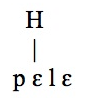
\includegraphics{../images/mende_house_a.png}
\end{figure}

\newpage

{\large Question 2}\\

Source: Final Exam Dataset\\

Explain how you would go about figuring out what to analyse in this dataset.\\

\begin{figure}[H]
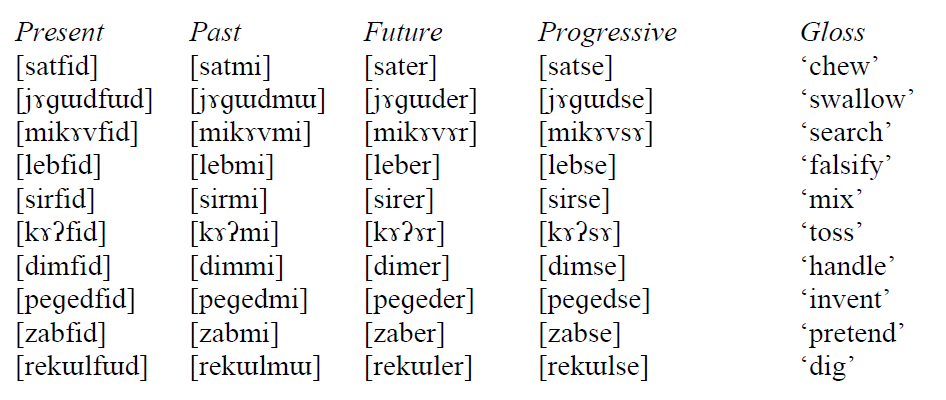
\includegraphics{../images/final_dataset.png}
\end{figure}

\newpage

{\large Question 3}\\

Source: Quiz 7, Question 8\\

Based on this data from Lamba, explain why the pair given below either does or does not show that the consonants preceding the morpheme for `with' are NOT responsible for the variation between [-il] and [-el].\\

čit-a \& čit-il-a

\begin{figure}[H]
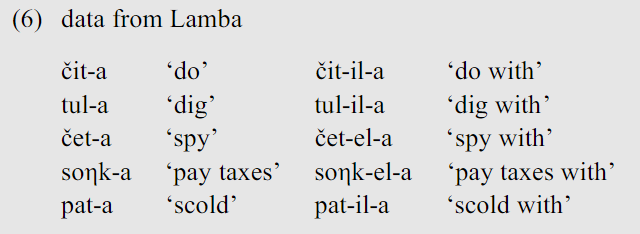
\includegraphics{../images/peng119_lamba.png}
\end{figure}

\newpage

{\large Question 4}\\

Source: Day 11 Handout, Question 10\\

Explain why this structure either is or is not a correct application of the templatic-based approach to syllabification, using the provided template and assuming that syllabification proceeds from left to right.\\

\begin{figure}[H]
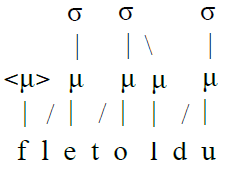
\includegraphics{../images/pengtemplate_fletoldu_no.png}
\end{figure}
\begin{figure}[H]
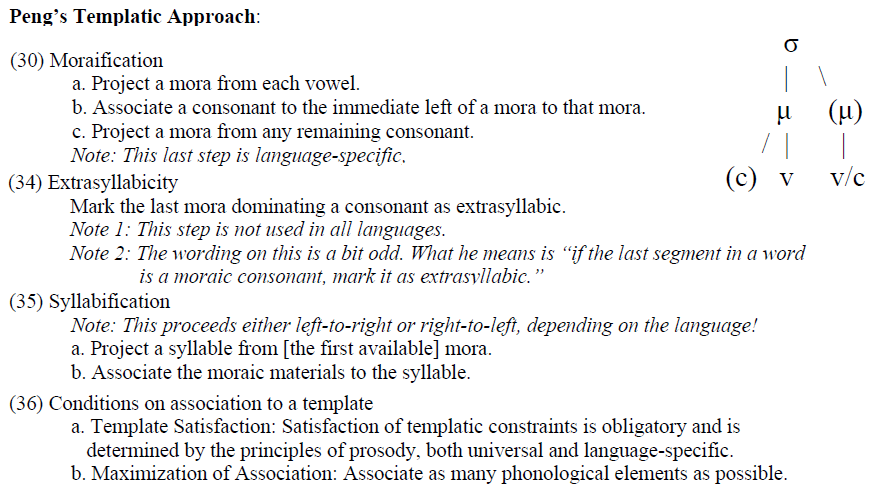
\includegraphics{../images/peng_template_withdiagram.png}
\end{figure}

\newpage

{\large Question 5}\\

Source: Quiz 6, Question 1\\

Explain what you see in the spectrogram that tells you about the properties of the sounds in the pictured word.\\

\begin{figure}[H]
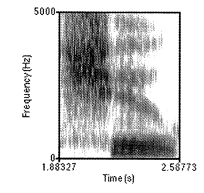
\includegraphics{../images/spectrogram_shoe.png}
\end{figure}

\newpage

{\large Question 6}\\

Source: Quiz 8, Question 3\\

Explain why this featural specification either does or does not match the given sound.\\

{[+consonantal]}, {[-sonorant]}

{[f]}


\newpage

\begin{center}
\textbf{{\color{red}{\HUGE END OF EXAM}}}\\

\end{center}
\newpage

\end{document}

